%
% One column figure
%-----------------------------------------------------------
   \begin{figure}
   \centering
\tikzstyle{smallfig}=[scale=0.25]
   %
   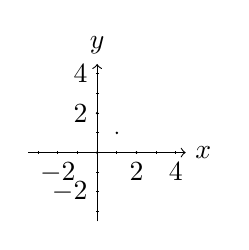
\begin{tikzpicture}[style=smallfig]
\draw[thin,->] (-3.5,0) -- (4.5,0) node[right] {$x$};
\draw[thin,->] (0,-3.5) -- (0,4.5) node[above] {$y$};

\foreach \x [count=\xi starting from 0] in {-3,-2,-1,,1,2,3,4}{% ticks
    \draw (\x,2pt) -- (\x,-2pt);
    \draw (2pt,\x) -- (-2pt,\x);
    \ifodd\xi
        \node[anchor=north] at (\x,0) {$\x$};
        \node[anchor=east] at (0,\x) {$\x$};
    \fi
}

\foreach \point in {(0,0),(0,2),(2,0),(1,1)}{% points
    \fill \point circle (2pt);
}

\end{tikzpicture}
\quad
\begin{tikzpicture}[style=smallfig]
\draw[thin,->] (-3.5,0) -- (4.5,0) node[right] {$x$};
\draw[thin,->] (0,-3.5) -- (0,4.5) node[above] {$y$};

\draw[dashed,thin,-] (0,3.0) -- (2,3.0);

\end{tikzpicture}
\quad
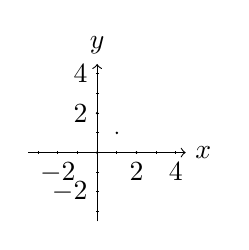
\begin{tikzpicture}[style=smallfig]
\draw[thin,->] (-3.5,0) -- (4.5,0) node[right] {$x$};
\draw[thin,->] (0,-3.5) -- (0,4.5) node[above] {$y$};

\foreach \x [count=\xi starting from 0] in {-3,-2,-1,,1,2,3,4}{% ticks
    \draw (\x,2pt) -- (\x,-2pt);
    \draw (2pt,\x) -- (-2pt,\x);
    \ifodd\xi
        \node[anchor=north] at (\x,0) {$\x$};
        \node[anchor=east] at (0,\x) {$\x$};
    \fi
}

\foreach \point in {(0,0),(0,2),(2,0),(1,1)}{% points
    \fill \point circle (2pt);
}

\end{tikzpicture}
   %
   \caption{The three symmetrical copies of $f$.}
   \label{fig:symms}
   \end{figure}
%-----------------------------------------------------------
%